\documentclass[margin=2mm]{standalone}
\usepackage{tikz}
\usetikzlibrary{decorations.pathreplacing, positioning}
\begin{document}
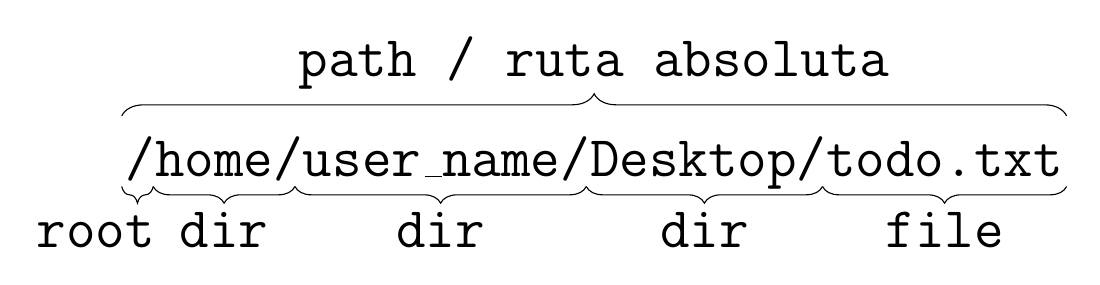
\begin{tikzpicture}[x=10mm, y=10mm, every node/.style={font=\ttfamily\huge}]
    \node (root) at (0,2) {/home/user\_name/Desktop/todo.txt};
    \draw[decorate, decoration={brace, amplitude=8}, yshift=0.7cm] (-6,1.9) -- (6,1.9) node[midway, above=6pt] {path / ruta absoluta};
    \draw[decorate, decoration={brace, mirror, amplitude=6}, yshift=20] (-6,1) -- (-5.6,1) node[midway, above=-0.9, xshift=-15] {root};
    \draw[decorate, decoration={brace, mirror, amplitude=6}, yshift=20] (-5.6,1) -- (-3.8,1) node[midway, above=-0.9] {dir};
    \draw[decorate, decoration={brace, mirror, amplitude=6}, yshift=20] (-3.8,1) -- (-0.1,1) node[midway, above=-0.9] {dir};
    \draw[decorate, decoration={brace, mirror, amplitude=6}, yshift=20] (-0.1,1) -- (2.9,1) node[midway, above=-0.9] {dir};
    \draw[decorate, decoration={brace, mirror, amplitude=6}, yshift=20] (2.9,1) -- (6,1) node[midway, above=-0.9] {file};
\end{tikzpicture}
\end{document}
